% Generated by pysimcount.pfseeds -- do not edit; regenerate instead.
% figure: B-all-by-formula -- Every formula at measured r; median over seeds [1, 2, 3, 4, 5, 6, 7, 8, 9, 10], bars = min..max
% metric=t gatebase=ct merged
% seed 1: git_commit=01d3c275ceae2840002bd1aaea68f59b987c4975 git_dirty=False
% seed 2: git_commit=01d3c275ceae2840002bd1aaea68f59b987c4975 git_dirty=False
% seed 3: git_commit=01d3c275ceae2840002bd1aaea68f59b987c4975 git_dirty=False
% seed 4: git_commit=01d3c275ceae2840002bd1aaea68f59b987c4975 git_dirty=False
% seed 5: git_commit=01d3c275ceae2840002bd1aaea68f59b987c4975 git_dirty=False
% seed 6: git_commit=01d3c275ceae2840002bd1aaea68f59b987c4975 git_dirty=False
% seed 7: git_commit=01d3c275ceae2840002bd1aaea68f59b987c4975 git_dirty=False
% seed 8: git_commit=01d3c275ceae2840002bd1aaea68f59b987c4975 git_dirty=False
% seed 9: git_commit=01d3c275ceae2840002bd1aaea68f59b987c4975 git_dirty=False
% seed 10: git_commit=01d3c275ceae2840002bd1aaea68f59b987c4975 git_dirty=False
% derived: B-all-by-formula.tex restyled by pysimcount.figuniform: extrapolated points (r from power-law fit) drawn in their series' measured style, style-key legend entries removed; extrapolated n = [13, 20]; source_sha256=b077fff29eaf5a7a07baab75bbac8a10afa0684731640bf3fe2585bd84926ef2
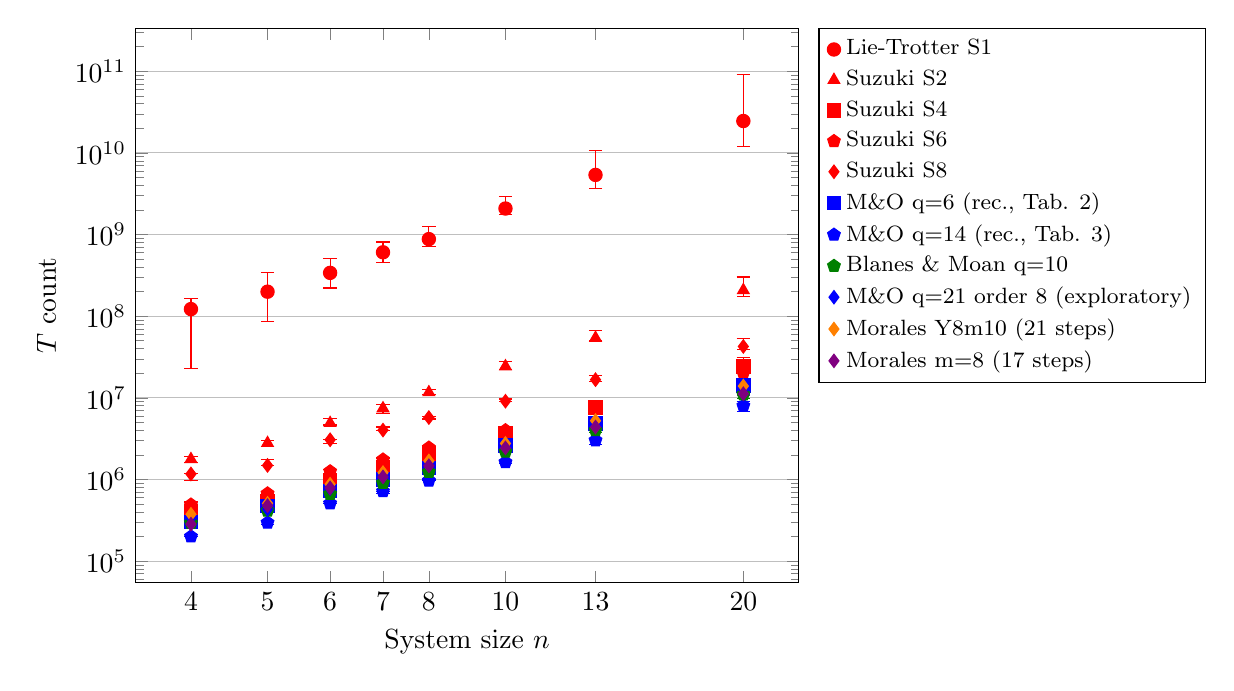
\begin{tikzpicture}
  \begin{loglogaxis}[
    width=10cm,
    xlabel={System size $n$},
    ylabel={$T$ count},
    xtick={4,5,6,7,8,10,13,20},
    xticklabels={4,5,6,7,8,10,13,20},
    ymajorgrids=true,
    legend pos=outer north east,
    legend cell align=left,
    legend style={font=\footnotesize},
  ]
    \addplot[only marks, red, mark=*, mark size=2.4pt, mark options={solid, fill=red}, error bars/.cd, y dir=both, y explicit, error bar style={red}] coordinates {
      (4,122032132) += (0,43012412) -= (0,98964458)
      (5,199402167) += (0,141546483) -= (0,114415587)
      (6,339047007) += (0,166002525) -= (0,117870207)
      (7,606237382) += (0,204620666) -= (0,155004910)
      (8,879209894) += (0,377799882) -= (0,162092340)
      (10,2082317356) += (0,862076772) -= (0,344145796)
    };
    \addlegendentry{Lie-Trotter S1}
    \addplot[only marks, red, mark=*, mark size=2.4pt, mark options={solid, fill=red}, forget plot, error bars/.cd, y dir=both, y explicit, error bar style={red}] coordinates {
      (13,5375044845) += (0,5310027219) -= (0,1702392705)
      (20,24572872883) += (0,66858476181) -= (0,12697597343)
    };
    \addplot[only marks, red, mark=triangle*, mark size=2.4pt, mark options={solid, fill=red}, error bars/.cd, y dir=both, y explicit, error bar style={red}] coordinates {
      (4,1770918) += (0,147882) -= (0,145186)
      (5,2788988) += (0,226588) -= (0,232918)
      (6,4900920) += (0,623180) -= (0,259036)
      (7,7419156) += (0,797708) -= (0,1059272)
      (8,11673189) += (0,947219) -= (0,761365)
      (10,24258489) += (0,3492291) -= (0,2298411)
    };
    \addlegendentry{Suzuki S2}
    \addplot[only marks, red, mark=triangle*, mark size=2.4pt, mark options={solid, fill=red}, forget plot, error bars/.cd, y dir=both, y explicit, error bar style={red}] coordinates {
      (13,54054476) += (0,12119840) -= (0,4232192)
      (20,208003079) += (0,94302923) -= (0,31889559)
    };
    \addplot[only marks, red, mark=square*, mark size=2.4pt, mark options={solid, fill=red}, error bars/.cd, y dir=both, y explicit, error bar style={red}] coordinates {
      (4,412976) += (0,1636) -= (0,14760)
      (5,535040) += (0,32200) -= (0,18800)
      (6,944950) += (0,72670) -= (0,49600)
      (7,1401914) += (0,62182) -= (0,84474)
      (8,2059726) += (0,70194) -= (0,107298)
      (10,3733848) += (0,423458) -= (0,39068)
    };
    \addlegendentry{Suzuki S4}
    \addplot[only marks, red, mark=square*, mark size=2.4pt, mark options={solid, fill=red}, forget plot, error bars/.cd, y dir=both, y explicit, error bar style={red}] coordinates {
      (13,7564669) += (0,1247087) -= (0,436653)
      (20,24179760) += (0,6979914) -= (0,2903274)
    };
    \addplot[only marks, red, mark=pentagon*, mark size=2.4pt, mark options={solid, fill=red}, error bars/.cd, y dir=both, y explicit, error bar style={red}] coordinates {
      (4,490685) += (0,40671) -= (0,1131)
      (5,672686) += (0,38464) -= (0,1442)
      (6,1254729) += (0,64127) -= (0,81529)
      (7,1747975) += (0,52889) -= (0,148923)
      (8,2446500) += (0,93082) -= (0,3420)
      (10,3997843) += (0,318145) -= (0,196833)
    };
    \addlegendentry{Suzuki S6}
    \addplot[only marks, red, mark=pentagon*, mark size=2.4pt, mark options={solid, fill=red}, forget plot, error bars/.cd, y dir=both, y explicit, error bar style={red}] coordinates {
      (13,7514691) += (0,974349) -= (0,801299)
      (20,20063997) += (0,4611641) -= (0,2718045)
    };
    \addplot[only marks, red, mark=diamond*, mark size=2.4pt, mark options={solid, fill=red}, error bars/.cd, y dir=both, y explicit, error bar style={red}] coordinates {
      (4,1166916) += (0,3384) -= (0,192396)
      (5,1485150) += (0,266208) -= (0,2082)
      (6,3060110) += (0,6170) -= (0,317900)
      (7,4023349) += (0,360779) -= (0,14839)
      (8,5725226) += (0,217410) -= (0,217100)
      (10,9084018) += (0,580614) -= (0,10982)
    };
    \addlegendentry{Suzuki S8}
    \addplot[only marks, red, mark=diamond*, mark size=2.4pt, mark options={solid, fill=red}, forget plot, error bars/.cd, y dir=both, y explicit, error bar style={red}] coordinates {
      (13,16670469) += (0,2093523) -= (0,729797)
      (20,42551241) += (0,11351927) -= (0,3129601)
    };
    \addplot[only marks, blue, mark=square*, mark size=2.4pt, mark options={solid, fill=blue}, error bars/.cd, y dir=both, y explicit, error bar style={blue}] coordinates {
      (4,302600) += (0,12120) -= (0,38120)
      (5,468630) += (0,10674) -= (0,63054)
      (6,721242) += (0,23090) -= (0,43082)
      (7,1002051) += (0,56097) -= (0,61363)
      (8,1379246) += (0,175790) -= (0,69022)
      (10,2604576) += (0,120480) -= (0,205344)
    };
    \addlegendentry{M\&O q=6 (rec., Tab. 2)}
    \addplot[only marks, blue, mark=square*, mark size=2.4pt, mark options={solid, fill=blue}, forget plot, error bars/.cd, y dir=both, y explicit, error bar style={blue}] coordinates {
      (13,4828267) += (0,393873) -= (0,149249)
      (20,14213266) += (0,1487930) -= (0,810202)
    };
    \addplot[only marks, blue, mark=pentagon*, mark size=2.4pt, mark options={solid, fill=blue}, error bars/.cd, y dir=both, y explicit, error bar style={blue}] coordinates {
      (4,199740) += (0,60) -= (0,380)
      (5,295424) += (0,15496) -= (0,15672)
      (6,509056) += (0,30728) -= (0,1152)
      (7,715540) += (0,874) -= (0,40504)
      (8,966548) += (0,41496) -= (0,924)
      (10,1624174) += (0,64346) -= (0,53038)
    };
    \addlegendentry{M\&O q=14 (rec., Tab. 3)}
    \addplot[only marks, blue, mark=pentagon*, mark size=2.4pt, mark options={solid, fill=blue}, forget plot, error bars/.cd, y dir=both, y explicit, error bar style={blue}] coordinates {
      (13,3012480) += (0,162468) -= (0,309312)
      (20,7963132) += (0,983748) -= (0,1234620)
    };
    \addplot[only marks, green!50!black, mark=pentagon*, mark size=2.4pt, mark options={solid, fill=green!50!black}, error bars/.cd, y dir=both, y explicit, error bar style={green!50!black}] coordinates {
      (4,292400) += (0,800) -= (0,13784)
      (5,413028) += (0,484) -= (0,20874)
      (6,665550) += (0,1102) -= (0,24126)
      (7,904662) += (0,19118) -= (0,28118)
      (8,1234038) += (0,61890) -= (0,28222)
      (10,2187862) += (0,28082) -= (0,70838)
    };
    \addlegendentry{Blanes \& Moan q=10}
    \addplot[only marks, green!50!black, mark=pentagon*, mark size=2.4pt, mark options={solid, fill=green!50!black}, forget plot, error bars/.cd, y dir=both, y explicit, error bar style={green!50!black}] coordinates {
      (13,3998210) += (0,160390) -= (0,224462)
      (20,10999812) += (0,781452) -= (0,1141124)
    };
    \addplot[only marks, blue, mark=diamond*, mark size=2.4pt, mark options={solid, fill=blue}, error bars/.cd, y dir=both, y explicit, error bar style={blue}] coordinates {
      (4,338998) += (0,792) -= (0,550)
      (5,431486) += (0,42202) -= (0,726)
      (6,776512) += (0,49892) -= (0,1504)
      (7,1091664) += (0,68376) -= (0,63504)
      (8,1506077) += (0,35751) -= (0,34937)
      (10,2527798) += (0,199114) -= (0,50502)
    };
    \addlegendentry{M\&O q=21 order 8 (exploratory)}
    \addplot[only marks, blue, mark=diamond*, mark size=2.4pt, mark options={solid, fill=blue}, forget plot, error bars/.cd, y dir=both, y explicit, error bar style={blue}] coordinates {
      (13,4702618) += (0,486062) -= (0,335430)
      (20,12795346) += (0,2221934) -= (0,1927074)
    };
    \addplot[only marks, orange, mark=diamond*, mark size=2.4pt, mark options={solid, fill=orange}, error bars/.cd, y dir=both, y explicit, error bar style={orange}] coordinates {
      (4,373908) += (0,324) -= (0,420)
      (5,509288) += (0,624) -= (0,468)
      (6,873450) += (0,53180) -= (0,48338)
      (7,1211994) += (0,55162) -= (0,59074)
      (8,1683875) += (0,50585) -= (0,79043)
      (10,2759488) += (0,295802) -= (0,95534)
    };
    \addlegendentry{Morales Y8m10 (21 steps)}
    \addplot[only marks, orange, mark=diamond*, mark size=2.4pt, mark options={solid, fill=orange}, forget plot, error bars/.cd, y dir=both, y explicit, error bar style={orange}] coordinates {
      (13,5244750) += (0,585450) -= (0,387282)
      (20,13925864) += (0,3288788) -= (0,1482490)
    };
    \addplot[only marks, violet, mark=diamond*, mark size=2.4pt, mark options={solid, fill=violet}, error bars/.cd, y dir=both, y explicit, error bar style={violet}] coordinates {
      (4,283369) += (0,15191) -= (0,14661)
      (5,477480) += (0,30360) -= (0,1500)
      (6,786680) += (0,42820) -= (0,960)
      (7,1073295) += (0,1495) -= (0,56543)
      (8,1469043) += (0,60765) -= (0,1215)
      (10,2430855) += (0,81441) -= (0,3535)
    };
    \addlegendentry{Morales m=8 (17 steps)}
    \addplot[only marks, violet, mark=diamond*, mark size=2.4pt, mark options={solid, fill=violet}, forget plot, error bars/.cd, y dir=both, y explicit, error bar style={violet}] coordinates {
      (13,4381387) += (0,171399) -= (0,78087)
      (20,11224575) += (0,782625) -= (0,527147)
    };
  \end{loglogaxis}
\end{tikzpicture}
